\documentclass[]{beamer}
\usetheme[background=light]{moloch}

\usepackage[backend=biber,style=authortitle,dashed=false,url=false]{biblatex}
\usepackage{svg}
\usepackage{tabularx}
\usepackage{emoji}
\usepackage{minted}
\usepackage{ragged2e}
\usepackage{xmpmulti}

\definecolor{ref}{HTML}{000080}
\definecolor{links}{HTML}{0066CC}
\hypersetup{colorlinks,linkcolor=,citecolor=ref,urlcolor=links}

\addbibresource{references.bib}

\title{C++20 Modules Support in SonarQube}
\subtitle{How We Accidentally Became a Build System}
\date{March 19, 2025}
\author{Alejandro Álvarez Ayllón}
\titlegraphic{\vbox to 3em {\hfill\includesvg[height=2em]{logos/SonarDark.svg}}}

% No section nor subsection slides
%\AtBeginSection[]{}
%\AtBeginSubsection[]{}

\setminted{fontsize=\scriptsize}

\newbibmacro{string+url}[1]{%
  \iffieldundef{url}{#1}{\href{\thefield{url}}{#1}}}
\DeclareFieldFormat{title}{\usebibmacro{string+url}{\mkbibemph{#1}}}
\DeclareFieldFormat[unpublished]{title}{\usebibmacro{string+url}{\mkbibquote{#1}}}
\DeclareFieldFormat[misc]{title}{\usebibmacro{string+url}{\mkbibquote{#1}}}

\begin{document}

\begin{frame}[standout]
  \setbeamercolor{title}{bg=black, fg=white}
  \setbeamercolor{subtitle}{fg=lightgray}
  \setbeamercolor{author}{fg=white}
  \setbeamercolor{date}{fg=white}
  \titlepage
\end{frame}

\begin{frame}{About Me}
  \begin{block}{Alejandro Álvarez Ayllón \emoji{flag-spain}}
    Completed my Master's and PhD at the University of Cádiz.
  \end{block}
  \begin{block}{Now Staff Engineer at Sonar}
    \begin{itemize}
      \item Member of ``CFamily'' (C, C++ and Objective-C).
      \item Contributed to the support of C++20 modules.
    \end{itemize}
  \end{block}

  \begin{block}{Previously...}
    \begin{itemize}
      \item University of Geneva: Astronomy Department (Euclid consortium).
      \item CERN: File Transfer Service (FTS) for LHC experiments.
    \end{itemize}
  \end{block}
\end{frame}

\begin{frame}{About Sonar}
  \begin{block}{Sonar}
    \begin{itemize}
      \item Continuous inspection of code quality and security
      \item Supports >30 languages
      \item \approx 700 employees \emoji{flag-switzerland} \emoji{flag-united-states} \emoji{flag-united-kingdom} \emoji{flag-singapore} \emoji{flag-germany} \emoji{flag-france}
      \item SonarQube \\
            \vspace{0.5em}
            \small \begin{tabular}{l l r}
              \href{https://www.sonarsource.com/open-source-editions/sonarqube-community-edition/}{Community} & Free and Open-source Platform                 &                                                           \\ \vspace{0.2em}
              \href{https://www.sonarsource.com/products/sonarqube/}{Server}                                  & On-premises installation                      & \raisebox{-.25\height}{\includesvg[width=1em]{logos/C++}} \\ \vspace{0.2em}
              \href{https://sonarcloud.io/login}{Cloud}                                                       & Cloud-based service, free for public projects & \raisebox{-.25\height}{\includesvg[width=1em]{logos/C++}} \\ \vspace{0.2em}
              \href{https://www.sonarsource.com/products/sonarlint/}{For IDE}                                 & VSCode, Visual Studio, IntelliJ, Eclipse      & \raisebox{-.25\height}{\includesvg[width=1em]{logos/C++}} \\
            \end{tabular}
    \end{itemize}
  \end{block}
\end{frame}

\begin{frame}{What to Expect}
  \begin{block}{}
    \begin{itemize}
      \item A retrospective on \emph{our} experiences adding C++20 modules support.
      \item Not a tutorial on C++20 modules.
            \begin{itemize}
              \item \cite{Weis24}
              \item I will give an overview of them, but I will not go into details.
            \end{itemize}
    \end{itemize}
  \end{block}
\end{frame}

\section{Brief Refresher on C++ Modules}
\begin{frame}[containsverbatim]{Before C++20}
  \begin{columns}
    \begin{column}{0.5\textwidth}
      \begin{block}{library.h}
        \inputminted{cpp}{snippets/cpp17/library.h}
      \end{block}
      \begin{block}{library.cpp}
        \inputminted{cpp}{snippets/cpp17/library.cpp}
      \end{block}
    \end{column}
    \begin{column}{0.5\textwidth}
      \begin{block}{main.cpp}
        \inputminted{cpp}{snippets/cpp17/main.cpp}
      \end{block}
    \end{column}
  \end{columns}
  \begin{block}{}
    \inputminted{bash}{snippets/cpp17/build.sh}
  \end{block}

  \note[item]{Compilation units are independent.}
  \note[item]{Compilation is parallelizable.}
  \note[item]{If there were more TU depending on \texttt{library.h}, they could be compiled in parallel.}
  \note[item]{But library.h has to be parsed every time, including its string include.}
\end{frame}


\begin{frame}[containsverbatim]{Since C++20}
  \begin{columns}
    \begin{column}{0.5\textwidth}
      \begin{block}{library.cppm}
        \inputminted{cpp}{snippets/cpp20/library.cppm}
      \end{block}
    \end{column}
    \begin{column}{0.5\textwidth}
      \begin{block}{main.cpp}
        \inputminted{cpp}{snippets/cpp20/main.cpp}
      \end{block}
    \end{column}
  \end{columns}
  \begin{block}{}
    \inputminted{bash}{snippets/cpp20/build.sh}
  \end{block}

  \note[item]{Now, if library is used from multiple TUs, it is parsed only once.}
\end{frame}

% Some main differences

% Terminology
\begin{frame}[containsverbatim]{Terminology}
  \begin{columns}
    \begin{column}{0.5\textwidth}

      \begin{block}{\footnotesize Global Module Fragment}
        \begin{minted}{cpp}
module;
// THIS is the GMF
// Only preprocessor directives
[export] module <identifier>;
    \end{minted}
      \end{block}

      \begin{block}{\footnotesize Primary Module Interface Unit}
        \begin{minted}{cpp}
export module <identifier>;
// Declarations
    \end{minted}
      \end{block}

      \begin{block}{\footnotesize Module Implementation Unit}
        \begin{minted}{cpp}
module <identifier>;

export import :part1;
export import :part2;
// Declarations
        \end{minted}
      \end{block}
    \end{column}

    \begin{column}{0.5\textwidth}

      \begin{block}{\footnotesize Module Interface Partition}
        \begin{minted}{cpp}
export module <identifier>:part1;
// Declarations
        \end{minted}
      \end{block}

      \begin{block}{\footnotesize Private Module Fragment}
        \begin{minted}{cpp}
export module <identifier>;
// Declarations

module : private;
// _Unreachable_ Declarations
        \end{minted}
      \end{block}

    \end{column}

  \end{columns}
\end{frame}

\begin{frame}[t,containsverbatim]{Terminology}

  \begin{columns}[t]
    \begin{column}{0.3\textwidth}
      \begin{block}{\footnotesize Attachment}
        \justifying \footnotesize If a declaration appears after the module declaration, it is attached to the module.
      \end{block}
    \end{column}

    \begin{column}{0.3\textwidth}
      \begin{block}{\footnotesize Module Linkage}
        \justifying   \footnotesize If attached to a named module but not exported.
      \end{block}
    \end{column}

    \begin{column}{0.3\textwidth}
      \begin{block}{\footnotesize Ownership Model}
        \justifying \footnotesize \textbf{Strong} if the module is part of the mangled name. \textbf{Weak} otherwise.
      \end{block}
    \end{column}
  \end{columns}

  \vspace{0.5em}

  \begin{columns}
    \begin{column}{0.5\textwidth}
      \begin{minted}{cpp}
export module foo;

// Attached to foo.
// Module linkage (`bar@foo`')
int bar();

// Attached to foo, external linkage.
// `::baz@foo` => Strong ownership.
// `::baz` => Weak ownership.
export int baz();
\end{minted}
    \end{column}
    \begin{column}{0.5\textwidth}
      \begin{minted}{cpp}
export module bar;

// Attached to bar.
// Module linkage (`bar@foo`'), OK.
int bar();

// Attached to bar, external linkage.
// `::baz@bar` => OK.
// `::baz` => ODR violation.
export int baz();
  \end{minted}
    \end{column}
  \end{columns}
\end{frame}

\begin{frame}[containsverbatim]{Terminology}
  \begin{columns}
    \begin{column}{0.5\textwidth}
      \begin{block}{\footnotesize Visibility}
        \footnotesize Can it be named from outside?
      \end{block}
    \end{column}
    \begin{column}{0.5\textwidth}
      \begin{block}{\footnotesize Reachability}
        \footnotesize Can it be reached from a visibible declaration?
      \end{block}
    \end{column}

  \end{columns}

  \vspace{0.5em}

  \begin{minted}{cpp}
export module foo;

export int a;           // Visible

int b () { return 0; }; // Not visible, module linkage

struct Foo {};          // Not visible, but reachable

export namespace bar {  // Visible
  Foo frobnicate() { return Foo {}; } // Visible, external linkage
}
  \end{minted}

  \vspace{0.5em}

  \small \cite{Engert21}

\end{frame}

\begin{frame}{Terminology}
  \begin{block}{}
    \textbf{BMI} Binary Module Interface \\
    \textbf{CMI} Compiled Module Interface

    \vspace{1em}

    Basically  a memory dump of the compiler internal representation of a module AST.

    They need to be built before the module can be imported.

    They are \emph{not} portable. Compiler, version, and even flags can affect them.
  \end{block}
\end{frame}

\begin{frame}{File Name and Extensions}
  Names are not meaningful, an extensions are purely a convention.

  \begin{itemize}
    \item \texttt{module.cppm} is preferred by clang.
    \item \texttt{module.cpp} is preferred by gcc.
    \item \texttt{module.ixx} is preferred by msvc.
  \end{itemize}

  But they don't matter much if the right flags are used.
  \note[item]{The extension is used by the compilers to automatically enable the corresponding flags.}
  \note[item]{This is relevant for the analyzer as well! We can not rely on the extension.}
\end{frame}

\begin{frame}[containsverbatim]{Terminology}
  \begin{block}{Header Units}
    \begin{minted}[fontsize=\normalsize]{cpp}
import <iostream>;
    \end{minted}
    \vspace{1em}
    Hard to use, hard to implement.
    \begin{itemize}
      \item \cite{Engert23}
      \item \cite{Ruoso23}
    \end{itemize}
  \end{block}
\end{frame}

% Requires build-system support (dependencies)
\begin{frame}{Build System Support}
  C++20 modules require build system support.
  \begin{itemize}
    \item Source files need to be scanned to find the dependencies.
    \item Modules need to be built before they can be imported.
    \item Compilation is \emph{not} embarransingly parallel anymore.
  \end{itemize}
\end{frame}

% Current status of compilers, libraries, etc.
\begin{frame}{Current Status}
  \begin{columns}[t]
    \begin{column}{0.5\textwidth}
      \begin{block}{Compilers}
        \small
        \begin{description}
          \item[GCC] Partial \note[item]{i.e. GCC does not implement private fragment}
          \item[Clang] Partial
          \item[MSVC] Complete
          \item[Apple Clang] No
        \end{description}
        Use the most recent version you can.
      \end{block}
    \end{column}

    \begin{column}{0.5\textwidth}
      \begin{block}{\texttt{import std;}}
        \small
        \begin{description}
          \item[libstdc++] Partial (\ge 15)
          \item[libc++] Partial (\ge 17)
          \item[MSSTL] Yes (\ge 17.5)
        \end{description}
      \end{block}
    \end{column}
  \end{columns}

  \vspace{1em}

  \begin{block}{Build Systems}
    \href{https://build2.org/}{build2}, \href{https://cmake.org/}{CMake},
    \href{https://learn.microsoft.com/en-us/visualstudio/msbuild/msbuild-command-line-reference?view=vs-2022}{MSBuild}
    and \href{https://xmake.io/}{xmake} support modules.
  \end{block}
\end{frame}

% We take code, analyzer it (duh!)
% Need to build the context.
% Tease about autoscan
\begin{frame}[t]{About the CFamily Analyzer}
  \begin{block}{}
    \begin{itemize}
      \item C, C++, Objective-C.
      \item Built on top of a fork of \href{https://clang.llvm.org/}{Clang} (19 as of today).
      \item We analyze the code \emph{how it was compiled}. We need to know
            \begin{itemize}
              \item The Compiler.
              \item The C++ standard.
              \item The include paths.
              \item The flags.
              \item The defines.
            \end{itemize}
      \item We leverage \texttt{compile\_commands.json}
            \begin{itemize}
              \item Generated by the build tools.
              \item Or by the \texttt{build-wrapper}.
            \end{itemize}
      \item We can also figure out some of these things \href{https://docs.sonarsource.com/sonarqube-cloud/advanced-setup/automatic-analysis}{automatically} \note{This will be relevant later}
    \end{itemize}
  \end{block}
  \note[item]{PVS Studio has \texttt{pvs-studio-analyzer trace}}
  \note[item]{Coverity has \texttt{cov-build}}
  \note[item]{Klocwork has \texttt{kwinject}}
\end{frame}

% We need to know how it is compiled (why?)
\begin{frame}[containsverbatim]{\texttt{compile\_commands.json}}
  \inputminted[breaklines]{json}{snippets/compdb/compile_commands.json}
  \begin{minted}{bash}
# These are generated when building
# std.cppm.o.modmap
-x c++-module -fmodule-output=CMakeFiles/__cmake_cxx23.dir/std.pcm
# main.cpp.o.modmap
-fmodule-file=std=CMakeFiles/__cmake_cxx23.dir/std.pcm
  \end{minted}
  \note{Wait, how do we generate the map? We need that. Hold that thought.}
\end{frame}

% Compilation database
% Build Wrapper

\section*{Let's Add Support for Modules!}

% Why now
%   Compiler & build system implementations starting to be usable, and converge on behavior (i.e. strong ownership)
%   We didn't want to implement something that could break in a month
%   We see low adoption, but of course, we do not support it. Nonetheless, not many requests either.
%   Anyway, let's add to the momentum, it seems a good moment.
\begin{frame}{Why now?}
  \begin{itemize}
    \item CMake support stopped being experimental by 3.28 (October 2023).
    \item Clang 19 was to be branched in Summer 2024.
          \begin{itemize}
            \item We need \texttt{-fmodules-reduced-bmi} for the feature to be usable.
            \item It purges unreachable entities from the BMI's.
          \end{itemize}
    \item The implementations are starting to be usable and stabilize.
  \end{itemize}
\end{frame}

\begin{frame}{Projects to test}
  \begin{itemize}
    \item \href{https://tinyurl.com/rwd48zpb}{SourceGraph query} for \texttt{export  module}, 87 hits.
    \item \href{https://tinyurl.com/ejey2pnt}{SourceGraph query} for \texttt{import}, 48 hits.
    \item Not great, many are toy examples, or test suites (i.e. gcc or llvm).
  \end{itemize}
  \begin{figure}
    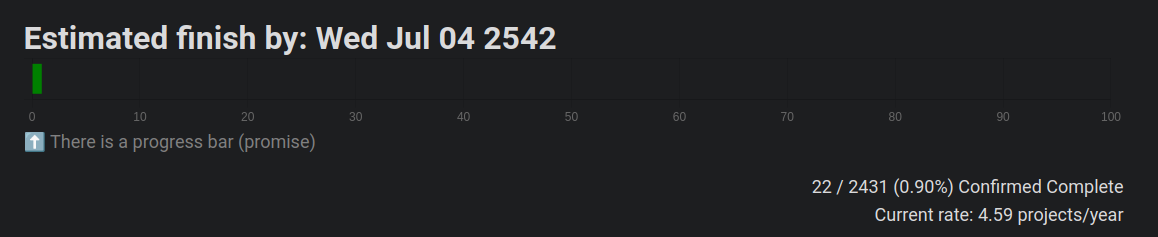
\includegraphics[width=\linewidth]{arewemodules.png}
    \caption{\href{https://arewemodulesyet.org/}{Are we modules yet?}}
  \end{figure}
\end{frame}

\begin{frame}{Projects to test}
  Nonetheless, we found some interesting ones:
  \begin{itemize}
    \item \href{https://github.com/infiniflow/infinity}{Infinity}, and AI database.
    \item \href{https://github.com/mpusz/mp-units}{mp-units}, quantities and units library (proposed for C++29).
    \item \href{https://github.com/alibaba/async_simple/tree/CXX20Modules}{async\_simple}, library of asynchronous components.
    \item And a few others.
  \end{itemize}
\end{frame}

% Dependencies
\begin{frame}{First things first}
  We need to know who exports and imports what.
  \begin{itemize}
    \item Names are not meaningful. Extensions aren't either.
    \item Can we use the compilation database?
  \end{itemize}
\end{frame}

\begin{frame}{First things first}
  \begin{block}{msvc \emoji{smile}}
    \footnotesize{
    \texttt{/TP /interface /ifcOutput {\color{red} mod.pcm} /Fo:mod.obj {\color{blue}mod-source.cppm}} \\
    \texttt{/reference {\color{purple}mod=mod.pcm} /Fo:main.obj {\color{blue}main.cpp}}
    }
  \end{block}
  \begin{block}{clang \emoji{smile}}
    \footnotesize{
    \texttt{-x c++-module -fmodule-output={\color{red}mod.pcm} -o mod.o {\color{blue}mod-source.cppm}} \\
    \texttt{-fmodule-file={\color{purple}mod=mod.pcm} -o main.o {\color{blue}main.cpp}}
    }
  \end{block}
  \begin{block}{gcc \emoji{neutral-face}}
    \footnotesize{
    \texttt{-fmodule-mapper={\color{magenta}mod.mm} -o mod.o -x c++ {\color{blue}mod-source.cppm}} \\
    \texttt{-fmodule-mapper={\color{magenta}mod.mm} -o main.o {\color{blue} main.cpp}}
    }
  \end{block}
\end{frame}

\begin{frame}{First things first}
  \begin{block}{msvc \emoji{unamused-face}}
    \footnotesize{
    \texttt{/TP /interface {\color{magenta}/ifcOutput modules} /Fo:mod.obj {\color{blue} mod-source.cppm}} \\
    \texttt{{\color{magenta}/ifcSearchDir modules} /Fo:main.obj main.cpp}
    }
  \end{block}
  \begin{block}{clang \emoji{unamused-face}}
    \footnotesize{
    \texttt{-x c++-module -fmodule-output={\color{red}mod.pcm} -o mod.o {\color{blue}mod-source.cppm}} \\
    \texttt{{\color{magenta}-fprebuilt-module-path=.} main.cpp}
    }
  \end{block}
\end{frame}

%   Forget it, scan dependencies!
\begin{frame}{First things first}
  Forget it, we'll scan the dependencies.
  \begin{itemize}
    \item Involves only the preprocessor, so it can be done quickly.
    \item We can do it in parallel.
    \item Infinity: Less than 7 seconds for 1\,485 files with 16 cores (full analysis lasts 1h 12 minutes) \emoji{pinching-hand}.
  \end{itemize}
  \note{We have re-invented \texttt{clang-scan-deps}, which is what CMake uses for clang and modules.}
\end{frame}

\begin{frame}[containsverbatim]{First things first}
  After scanning, we have a list of who-provides-what, and who-needs-what.
  \begin{block}{}
    \footnotesize{
    \texttt{{\color{blue}stl}=src/common/stl.cppm: []\\
    {\color{blue}default\_values}=src/common/default\_values.cppm: [{\color{purple}stl}]\\
    {\color{blue}ring\_buffer\_iterator}=src/network/ring\_buffer\_iterator.cppm: [{\color{purple}stl, default\_values}]\\
    ...}
    }
  \end{block}
  We need to put together a graph.
\end{frame}

\begin{frame}{Dependency Graph}
  \small From a toy example so it fits in a slide.
  \begin{figure}
    \includegraphics[width=0.9\textwidth]{graph/ptraced.pdf}
  \end{figure}
\end{frame}

\begin{frame}{Building the BMI's}
  \multiinclude[<+->][format=pdf, graphics={width=\textwidth}]{graph/building/step}
\end{frame}

\begin{frame}{We can now analyze}
  \begin{itemize}
    \item We could analyze as we build the BMI's, but we decided to do it in two steps.
    \item Once we have the BMI's, we can parallelize the analysis to the maximum, which is more intensive.
  \end{itemize}
  \begin{block}{What do we do with the BMI's?}
    Infinity's take 2.61 GiB of disk space. Uploading/downloading them from the server is not a good option.

    They are transient, and we rebuild them when necessary.
    \note{And that's with the reduced BMI!}
  \end{block}
\end{frame}

\begin{frame}{Well, that's not efficient}
  \begin{block}{Differential Analysis}
    The CFamily analyzer does not analyze the whole project every time.
    Nor on the \texttt{main} branch, nor on PR's.
    \begin{itemize}
      \item We analyze only the files that changed.
      \item If a header changes, we analyze the files that include it.
    \end{itemize}
    We need to adapt this to our handling of modules.
  \end{block}
\end{frame}

\begin{frame}{Re-Building the BMI's}
  \multiinclude[<+->][format=pdf, end=2,graphics={width=\textwidth}]{graph/changed/step}
\end{frame}

\begin{frame}{Re-Building the BMI's \emoji{see-no-evil-monkey}}
  \includegraphics[width=\textwidth]{graph/changed/step-3.pdf}
\end{frame}


\begin{frame}{Differential Analysis}
  \begin{itemize}
    \item We ended rebuilding almost everything.
    \item We do \emph{not} re-analyze everything.
    \item That's how it is, we can't do much about it.
    \item On the bright side, for a clean scan of Infinity:
          \begin{itemize}
            \item 643 BMI's need to be built.
            \item I takes a bit over 2 minutes out of 1h 12 minutes (16 cores).
          \end{itemize}
  \end{itemize}
\end{frame}

\begin{frame}{We ended up having to}
  \begin{enumerate}
    \item Scan the source files to find \texttt{import} / \texttt{export} statements.
    \item Build the dependency graph.
    \item Traverse it in order to generate the BMI's.
    \item On incremental changes, implement the logic to:
          \begin{itemize}
            \item Re-build what is necessary to analyze the modified file.
            \item Re-analyze what is affected by the changes.
            \item Re-build what is necessary to analyze the files affected by the change \emoji{grimacing-face}.
          \end{itemize}
    \item Do all of this while trying to utilize the available cores efficiently.
  \end{enumerate}
  If we had code generation, we could almost build the program\footnote{\tiny Just kidding, this would only half-work for module-only projects.}.
\end{frame}

\begin{frame}{One take away?}
  \begin{figure}
    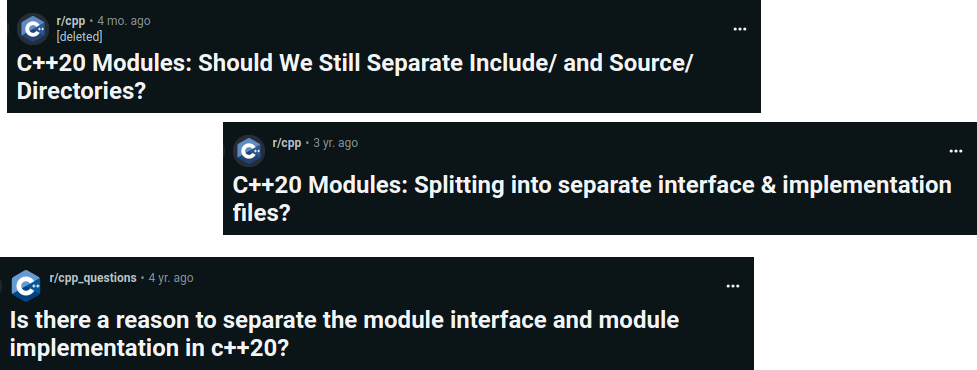
\includegraphics[width=\linewidth]{questions.png}
  \end{figure}
  \centering
  Probably yes.
\end{frame}

\section*{What About Ill-Formed Programs?}
% Wait, What? Why?
% Unsupported compilers / builtins (not much of a problem for the big three that support modules)
% AutoScan!
% We need to write BMIs from Ill-formed code
% Turns out clang is pretty resilient to this, but not perfect, quite a few crashes
%   Do they care? Maybe they do (clang-tidy, clangd)
%   Tooling probably cares in general about this aspect
\begin{frame}{Wait... what?}
  \begin{block}{Why?}
    Analyzers need to be more resilient to parsing errors.
    \begin{itemize}
      \item Unsupported compilers or unsupported builtins.
      \item Unsupported language features.
      \item \href{https://docs.sonarsource.com/sonarqube-cloud/advanced-setup/automatic-analysis}{Automatic Analysis}.
    \end{itemize}
  \end{block}
  Clang is already pretty resilient\footnote{Probably because of \texttt{clang-tidy} and \texttt{clangd}}, and can give an AST even for ill-formed programs.
\end{frame}

\begin{frame}[containsverbatim]{Example}
  \begin{columns}
    \begin{column}{0.4\textwidth}
      \begin{minted}{cpp}
int foo() {
    int i = 0;
    if (IForgotAnInclude()) {
        i += 1;
    }
    return i;
}
    \end{minted}
    \end{column}
    \begin{column}{0.6\textwidth}
      \tiny\texttt{
      TranslationUnitDecl \\
      `-FunctionDecl <line:2:1, line:8:1> line:2:5 foo 'int ()' \\
      `-CompoundStmt <col:11, line:8:1> \\
      |-DeclStmt <line:3:5, col:14> \\
      | `-VarDecl <col:5, col:13> col:9 used i 'int' cinit \\
      |   `-IntegerLiteral <col:13> 'int' 0 \\
      |-IfStmt <line:4:5, line:6:5> \\
      | |-{\color{red}RecoveryExpr <line:4:9, col:26> '<dependent type>' contains-errors} lvalue \\
      | | `-{\color{purple}UnresolvedLookupExpr <col:9> '<overloaded function type>' lvalue (ADL) = 'IForgotAnInclude' empty} \\
      | `-CompoundStmt <col:29, line:6:5> \\
      |   `-CompoundAssignOperator <line:5:9, col:14> 'int' lvalue '+=' ComputeLHSTy='int' ComputeResultTy='int' \\
      |     |-DeclRefExpr <col:9> 'int' lvalue Var 0x2a9dbc90 'i' 'int' \\
      |     `-IntegerLiteral <col:14> 'int' 1 \\
      `-ReturnStmt <line:7:5, col:12> \\
      `-ImplicitCastExpr <col:12> 'int' <LValueToRValue> \\
      `-DeclRefExpr <col:12> 'int' lvalue Var 0x2a9dbc90 'i' 'int'
      }
    \end{column}
  \end{columns}
  \vspace{1em}
  \begin{center}
    \small What if this was a module with an export?
  \end{center}
\end{frame}

\begin{frame}[t]{Modules with errors}
  \begin{block}{}
    \small Fortunately clang can emit and load BMI's with errors: \texttt{-fallow-pcm-with-compiler-errors}\footnote{Capability that was \href{https://github.com/llvm/llvm-project/pull/121485}{briefly gone between versions 19 and 20}.}.

    \vspace{0.5em}

    Unfortunately, there were some bugs lurking around, and there may still be:
    \begin{itemize}
      \item \href{https://github.com/llvm/llvm-project/pull/111179}{Don't evaluate concept when its definition is invalid}
      \item \href{https://github.com/llvm/llvm-project/pull/121550}{Do not serialize function definitions without a body.}
      \item \href{https://github.com/llvm/llvm-project/pull/121768}{Fix initialization of NonTypeTemplateParmDecl when there are invalid constraints.}
    \end{itemize}
  \end{block}
  \begin{block}{}
    \small Not necessarily all found bugs  were due to modules \emoji{sweat-smile}:
    \href{https://github.com/llvm/llvm-project/pull/118288}{Fix non-deterministic infinite recursion...} (mp-units)
  \end{block}
\end{frame}

\begin{frame}{What is missing?}
  \begin{block}{}
    \begin{enumerate}
      \item \texttt{import std;} for Automatic Analysis.
      \item Review rules that can be affected by modules. Some known \emph{False Positives}:
            \begin{itemize}
              \item \href{https://sonarsource.github.io/rspec/\#/rspec/S1000/cfamily}{S1000}: Header files should not contain unnamed namespaces
              \item \href{https://sonarsource.github.io/rspec/\#/rspec/S1003/cfamily}{S1003}: \texttt{using namespace} directives should not be used in header files
            \end{itemize}
            Adoption is still low, so hard to prioritize.
      \item SonarQube for IDE.
            \addtocounter{enumi}{95}
      \item Header units.
    \end{enumerate}
  \end{block}
\end{frame}

% Where is it supported?
\begin{frame}{Support}
  \begin{block}{}
    \begin{table}
      \begin{tabular}{m{10em}  p{3em}}
        \includesvg[width=8em]{logos/SQ_Logo_Cloud_Light Backgrounds}  & \emoji{green-circle} \\[1em]
        \includesvg[width=8em]{logos/SQ_Logo_Server_Light Backgrounds} & \emoji{green-circle}
      \end{tabular}
    \end{table}
  \end{block}
  \begin{block}{}
    \begin{table}
      \newcolumntype{Y}{>{\centering\arraybackslash}X}
      \begin{tabular}{m{10em} p{3em}}
        \includesvg[width=8em]{logos/SQ_Logo_IDE_Light Backgrounds} & \emoji{red-circle} \\[1.5em]
        \multicolumn{2}{c}{
          \begin{tabularx}{14em}{l Y Y r}
            \includesvg[width=1.5em]{logos/Clion} & \includesvg[width=1.5em]{logos/vscode} & \includesvg[width=1.5em]{logos/vs} & \includesvg[width=1.5em]{logos/eclipse} \\
            \multicolumn{4}{l}{} Different IDE's, different API's                                                                                                         \\
          \end{tabularx}
        }
      \end{tabular}
    \end{table}
  \end{block}
\end{frame}

\begin{frame}[standout]
  \centering
  \includesvg[width=0.2\textwidth]{logos/SonarMarkDark.svg}

  \huge Questions?
\end{frame}

\begin{frame}{More Material}
  \printbibliography[heading=none]
\end{frame}

\end{document}
